\documentclass{article}
\usepackage{amsmath}
\usepackage{amssymb}
\usepackage{geometry}
\usepackage{xcolor}
\usepackage{mdframed}
\geometry{a4paper, margin=1in, bottom=2cm}
\usepackage{tikz}
\usetikzlibrary{positioning}  % Biblioteca necesaria para "right of"
\usepackage{graphicx}
\usepackage{parskip}
\usepackage{caption}
\usepackage[spanish]{babel}

\title{Guía de Problemas: Árbol de Expansión Mínima y Flujo Máximo}
\author{Ricardo Largaespada}
\date{18 de marzo 2025}

\newmdenv[
  backgroundcolor=blue!5,
  linecolor=blue,
  linewidth=1pt,
  roundcorner=5pt,
  skipabove=\baselineskip,
  skipbelow=\baselineskip
]{problem}

\begin{document}

\maketitle

\begin{problem}
\textbf{Árbol de Expansión Mínima (MST)}

Dado un grafo ponderado y no dirigido, el objetivo es encontrar un árbol que conecte todos los nodos minimizando la suma total de los pesos de sus aristas. Este problema es fundamental en la optimización de redes.

\textbf{Tarea:}
\begin{enumerate}
    \item Aplicar el algoritmo de Kruskal para encontrar el MST del grafo.
    \item Aplicar el algoritmo de Prim para resolver el mismo problema.
    \item Comparar ambos métodos en términos de complejidad y escenarios de aplicación.
\end{enumerate}

\textbf{Ejemplo:} Considere el siguiente grafo:

\begin{center}
    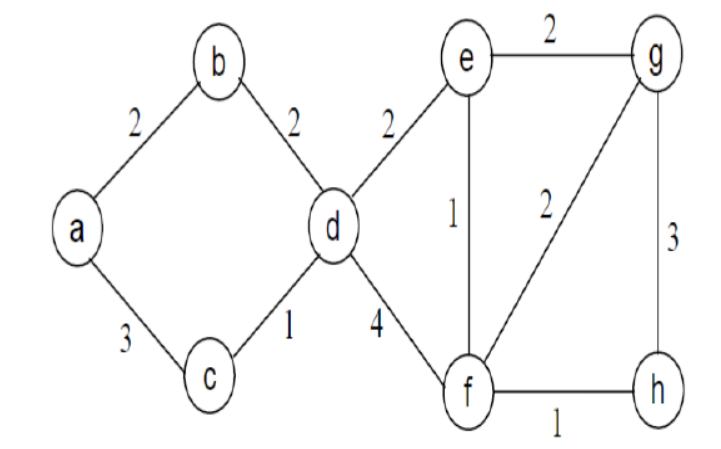
\includegraphics[scale=0.4]{images/trabajo02-1.png}
\end{center}
\end{problem}

\begin{problem}
\textbf{La maderera Wirehouse}\\

La maderera Wirehouse talará árboles en ocho zonas de la misma área. Pero antes debe desarrollar un sistema de caminos de tierra para tener acceso a cualquier zona desde cualquier otra. La distancia (en millas) entre cada par de zonas es la siguiente:

\begin{center}
\begin{tabular}{|c|c|c|c|c|c|c|c|c|}
\hline
Zona & 1 & 2 & 3 & 4 & 5 & 6 & 7 & 8 \\
\hline
1 & - & 1.3 & 2.1 & 0.9 & 0.7 & 1.8 & 2.0 & 1.5 \\
2 & 1.3 & - & 0.9 & 1.8 & 1.2 & 2.6 & 2.3 & 1.1 \\
3 & 2.1 & 0.9 & - & 2.6 & 1.7 & 2.5 & 1.9 & 0.6 \\
4 & 0.9 & 1.8 & 2.6 & - & 0.7 & 1.7 & 1.6 & 0.8 \\
5 & 0.7 & 1.2 & 1.7 & 0.7 & - & 1.2 & 1.1 & 0.5 \\
6 & 1.8 & 2.6 & 2.5 & 1.6 & 1.2 & - & 1.1 & 0.6 \\
7 & 2.0 & 2.3 & 1.9 & 1.5 & 1.1 & 1.1 & - & 0.5 \\
8 & 1.5 & 1.1 & 1.0 & 0.9 & 0.5 & 0.6 & 0.5 & - \\
\hline
\end{tabular}
\end{center}

El problema es determinar los pares de zonas entre los que deben construirse caminos para conectar todas con una longitud de caminos total mínima.

\textbf{a)} Describa cómo se ajusta este problema a la descripción del problema del árbol de expansión mínima.

\textbf{b)} Utilice el algoritmo de su elección para resolverlo.

\end{problem}

\begin{problem}
\textbf{Flujo Máximo en una Red de Transporte}

El problema de flujo máximo busca determinar la cantidad máxima de flujo que se puede enviar de una fuente a un sumidero en una red, respetando las capacidades de las aristas. Este problema es de gran importancia en redes de comunicación y transporte.

\textbf{Tarea:}
\begin{enumerate}
    \item Utilizar el algoritmo de Ford-Fulkerson para calcular el flujo máximo desde la fuente (O) hasta el sumidero (T).
    \item Mostrar la red residual resultante después de alcanzar el flujo máximo.
    \item Discutir posibles mejoras o ajustes en la red para aumentar la capacidad total.
\end{enumerate}

\textbf{Ejemplo:} Considere la siguiente red de flujo:

\begin{center}
    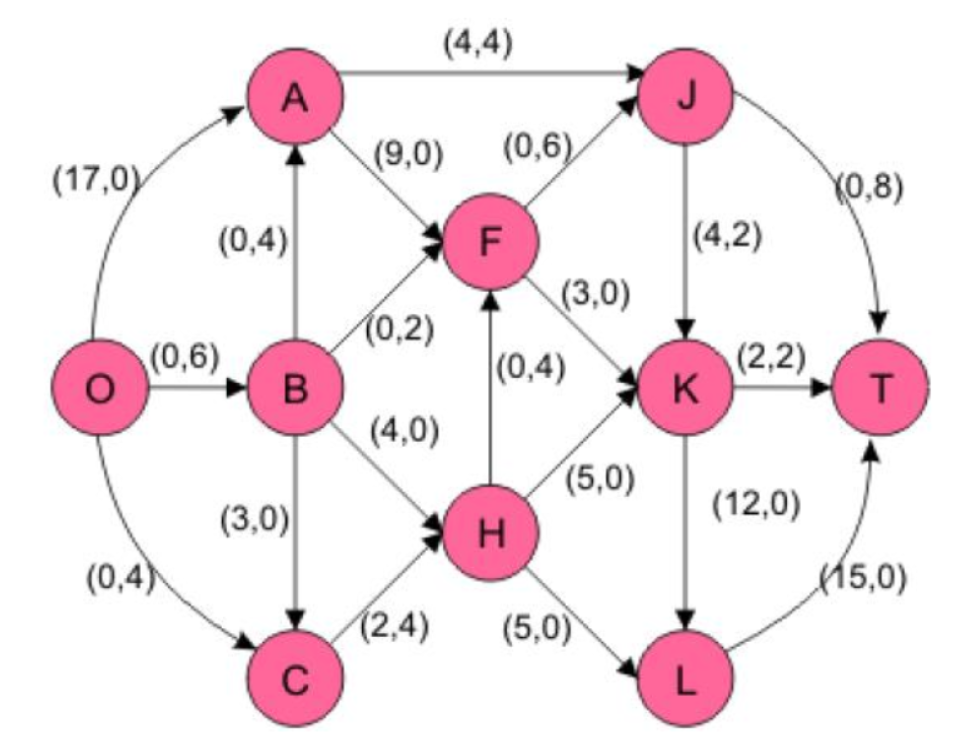
\includegraphics[scale=0.5]{images/trabajo02-2.png}
\end{center}
\end{problem}

\end{document}
